\section{Analysis of .bit domains}

In this section we analyze the current state of .bit domains. We explore the system on multiple levels. We begin at the highest level, looking at the repetition of values in order to detect squatters. Next we look at how many .bit domains are set up with query-able values. Finally we actually visit these query-able names and analyze the content we find there.

\subsection{Detecting Squatters}

We investigate the balance between squatters and other users in the .bit subspace. As we discussed in \ref{sec:model}, namespace squatting is an important issue to understand. We look at Namecoin in order to get a realistic view on the proliferation of squatting.

\begin{figure}
  \centering
  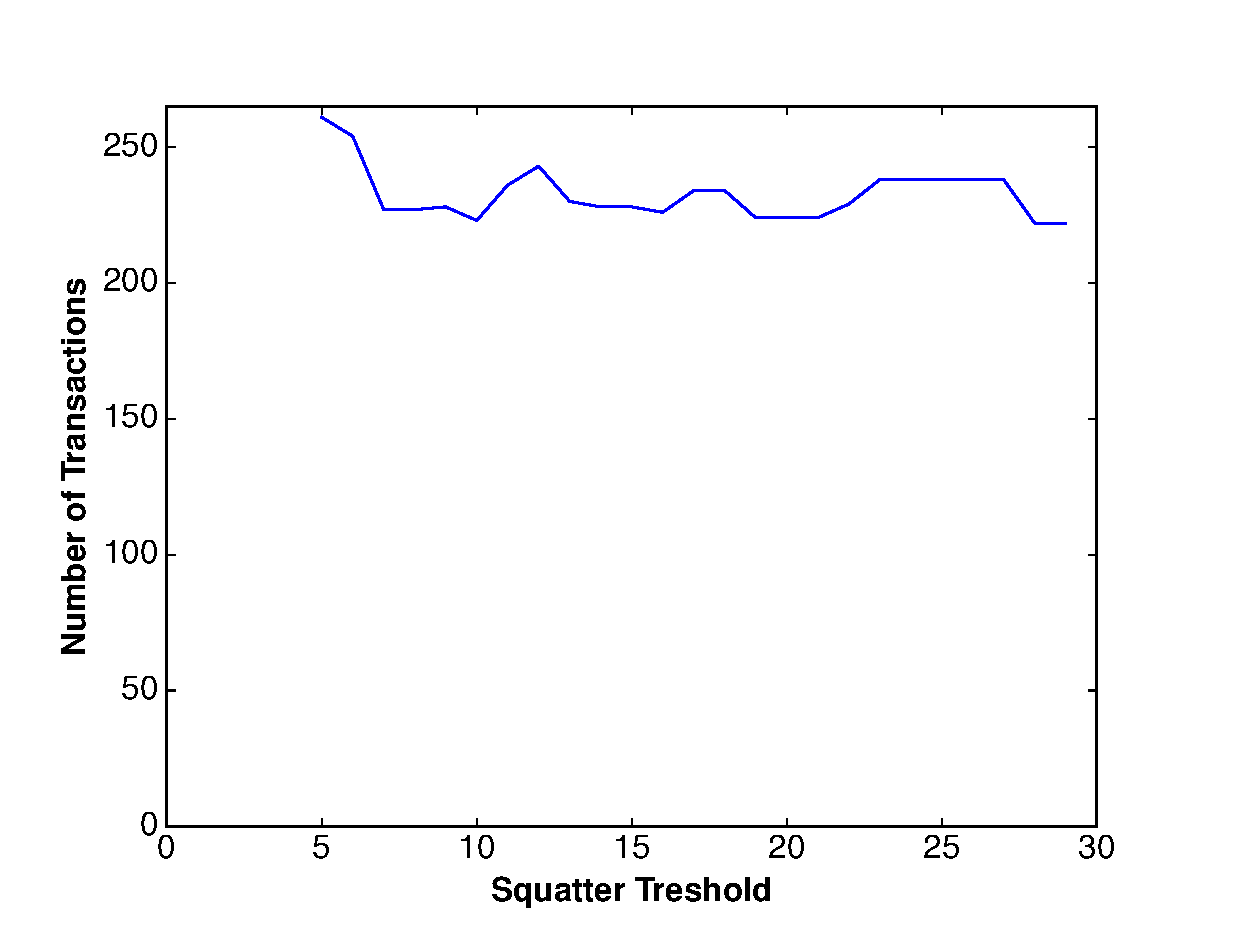
\includegraphics[width=0.9\columnwidth]{figures/squatters}
  \caption{Percent of names considered squatted}
  \label{fig:percentSquatter}
\end{figure}

Namecoin possesses the same pseudonymity properties as Bitcoin and thus it is difficult to group names by their owner. Names are owned by individual addresses rather than by identities and it is a common practice to keep each purchased name under a different address. Because of this, it is difficult to assess how many names a single person owns. 

However, many squatters are easily identified through the values they set on the names they own. Since there is no built-in functionality for the listing and sale of names in Namecoin, squatters use the values of names they own to display contact information. This information generally comes in the form of either contact information stored directly in the value of a name, or contact information stored at the IP address to which the name resolves.  We observed that a squatter's contact information is generally constant among all the names he owns. Thus, by measuring the extent to which values are duplicated on the block chain, we can estimate the rate of squatters compared to regular users.

Regular .bit domain owners are unlikely to use values that are highly replicated. The value of a domain points to an individual server and are mostly unique. The only repetition that may occur in this circumstance is when multiple names resolve to the same point. This could occur when a single DNS server is resolving a large number of names to different websites. However from our analysis in Section \ref{domainbreakdown}, we see that this does not happen currently.

There is no clear method for deciding exactly how often a value has to occur in order to assume a squatter has been detected. However even the coarsest grained approach displays a massive amount of squatting on the block chain. Simply observing the 196023 currently active names, reveals that there are only 34361 unique values.

In figure \ref{fig:percentSquatter} we examine the fraction of current .bit names that are squatted. We sorted all of the values that occur by the number of times they occur. 
%As the graph threshold moves along the X-axis, the sum of only values that occur more than $n$ times is show. 
The graph has a very sharp initial drop as we remove all names with values that occur only a few times. This leaves the majority of domains to drop off very slowly as we remove bigger and bigger squatters. Using a cut-off of $n=$\hi{[fill in]}, it appears safe to say that at least 70\% of .bit domains are held by squatters.

\subsection{DNS Records}

\begin{table}[t]
\begin{tabular}{ll}
Type of Resolution & Count \\ \hline
Nameserver URL     & 3359  \\
Nameserver IP      & 175   \\
Single IP          & 6304  \\
Multiple IP        & 3     \\
Single IPv6        & 3     \\
Multiple IPv6      & 1     \\
Tor                & 12    \\
Alias              & 27    \\
Only Subdomains    & 135   \\ \hline
Total              & 10019
\end{tabular}
\caption{.bit domain resolution methods}
\end{table}

We now examine how .bit domains are used by legitimate users. Only 10019 out of the 141422 .bit domains make any attempt to resolve to IP addresses. Out of these a variety of types of IP resolution are employed.

In order to support DNS lookups, Namecoin provides a specification that allows for the support of most DNS record types. A name's configuration is stored in a JSON dictionary object which is placed in a name's value. Domain's can be configured in a number of different ways. The main methods are directly setting one of more IP (or IPv6) addresses or setting one or more secondary name-servers which hold information about a domain. Additionally records can link a name to a number of hidden services like .onion \cite{onion} and .i2p \cite{i2p}.

Namecoin supports a number of different name resolution methods. Different methods have different properties and thus it is interesting to inspect how people are setting up their domains. The vast majority of people are pointing their domains directly to an address. This includes people using IP, IPv6, and Tor. This is by far the most secure method since the IP address is protected directly with block chain security. A user can simply look up a name in the block chain and immediately be linked to a server. However, this security comes at the cost of flexibility since the server is directly encoded in the block chain, and can not be changed without an update.


%insecure delegation like DNSSEC
% cite DNS lookup attack
The much more flexible configuration, used by a large number of people as well, is name server delegation. Rather than directly listing an IP address in the blockchain, one or more name servers are listed. This way a name owner can update its IP address without modifying the blockchain. However this is an insecure delegation since Namecoin can not enforce any security properties regarding the action of the external name server. Additionally if a name server is listed with a hostname rather than and IP address, a standard DNS lookup must occur, linking Namecoin with standard DNS.

\subsection{Domain Content Analysis}
\label{domainbreakdown}

w\begin{table}[t]
\begin{tabular}{ll}
Valid DNS          &  10019  \\
Curlable        & 5374     \\
Not Squatter        & 745     \\
Without Duplicates      & 455     \\
Without Errors              & 278    \\
With Content              & 222    \\
Without ICANN hostname   & 28   \\
\end{tabular}
\caption{Reduction of domains to real content}
\end{table}

After understanding how people connect their names with IP addresses, we explored what sort of content is reachable through .bit domain names. We attempted to download the www front page of each of these 10019 domains over port 80 (http). 4546 of these domains were unreachable or didn't serve web content, which left us with only 5374 domains which present any response.

At this point we moved to looking at the content of server responses. Immediately noticeable was that out of the 5374 domains with server responses, 4629 are owned by 3 different squatters. These domains hold nothing of value and caused massive inflation in our reachable domain count.

Without the squatters, we count 745 viable domains. However, many of these pages include identical content which does not add value to the system. After removing 290 of such duplicates, 455 domains remained.

At this point we started inspecting the actual content of the webpages. A large number of them were either error responses from the server or default pages from various servers. Neither of these types of pages are usable content. Removing the 177 of these left us with 278 domains.

Out of the remaining sites, many had very small amounts of content consisting of only a few words on a blank page like, "Welcome to mysite.bit." These pages, though valid uses of Namecoin, do not provide any utility to a visitor. Thus, we decided to look at only pages consisting of 15 or more words and images which brought us down to 222 domains.

These 222 domains make up the only websites reachable through .bit domain names which have real content on them at the time of this analysis. We are further interested in the subset of these pages which don't come from a server that is accessible through a standard ICANN TLD as well.  83 of the pages directly redirect the user to a standard domain and 111 were manually identified as pointing to the same site as a standard domain.

We finished our analysis with 28 pages remaining. These pages represent the .bit unique content available.

Our approach to analyzing content suffers from a few limitations. First of all we only queried the main domain over port 80, thus if any of the servers only respond to subdomains or only serve content over HTTPS, they are not included. Additionally when we detect how much content is on each page, we do not follow links and thus content could be hidden behind links. Despite these limitations we believe that we have missed very few legitimate domains.

\subsection{Categorizing Squatter Name Decisions}

\begin{figure}[t]
  \centering
  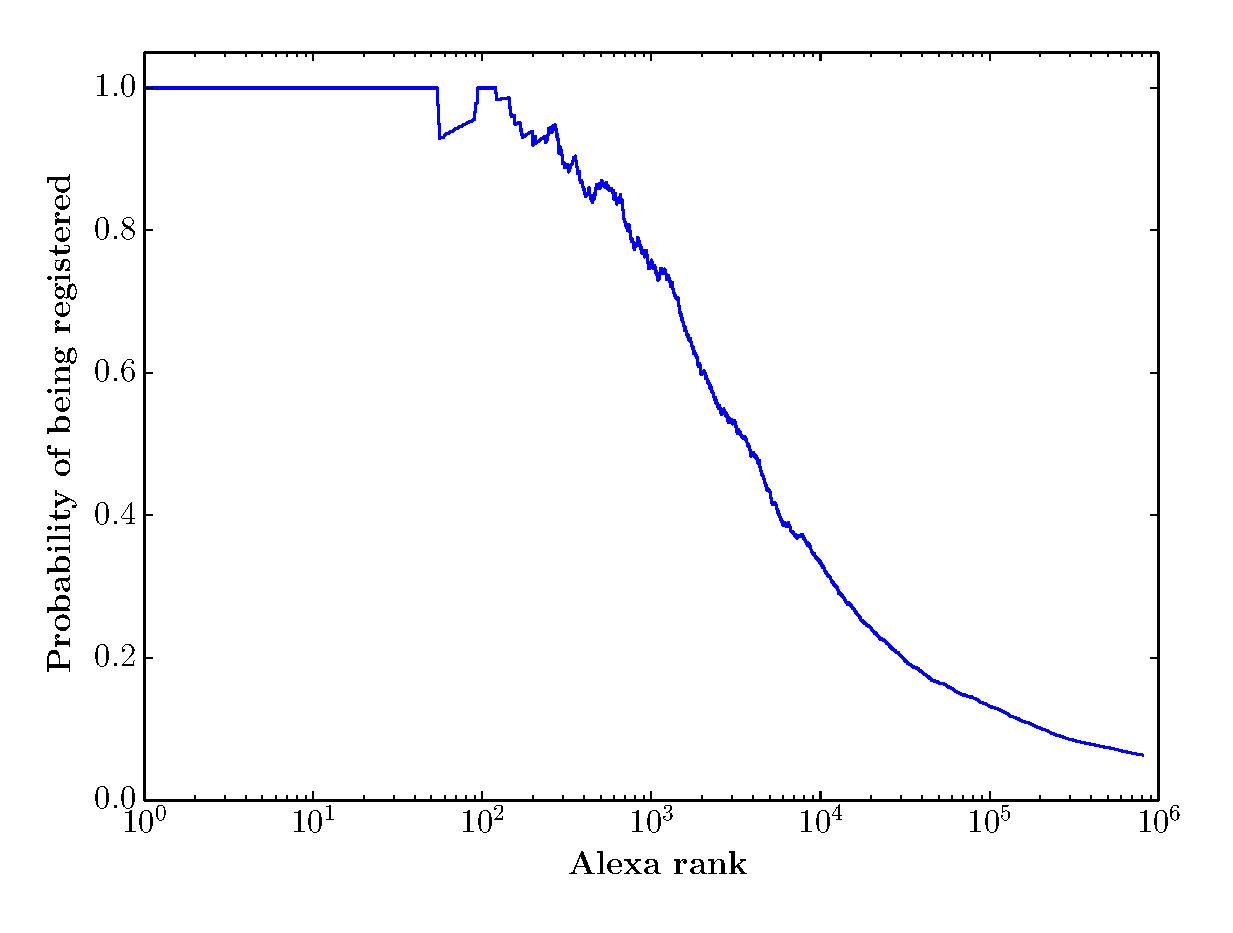
\includegraphics[width=\columnwidth]{figures/alexa_probability}
  \caption{The probability that a name that shows up on the Alexa top 1 million rank is registered given by the rank of the name.}
  \label{fig:alexa_probability}
\end{figure}

As we have seen, many individual squatters buy up very large numbers of domains. We now explore what sort of categories these names fall into and try to interpret the decisions these squatters have made.

We can see from Figure \ref{fig:alexa_probability} and Figure \ref{fig:name_length_histogram} that there are patterns to the names that squatters have acquired. In Figure \ref{fig:alexa_probability}, we can see that squatters have claimed the majority of very high ranking Alexa sites.

In Figure \ref{fig:name_length_histogram} we see that there is a preference for shorter names. Table \ref{table:names_available} shows that in fact all one and two character names are taken. It is not until we get to names with at least three characters are there names available to register. Beyond three characters, the combinatorial nature of name strings makes it infeasible to register all names of that length. There are more names with a length of 4 available than there are total names registered currently.


\begin{figure}
  \centering
  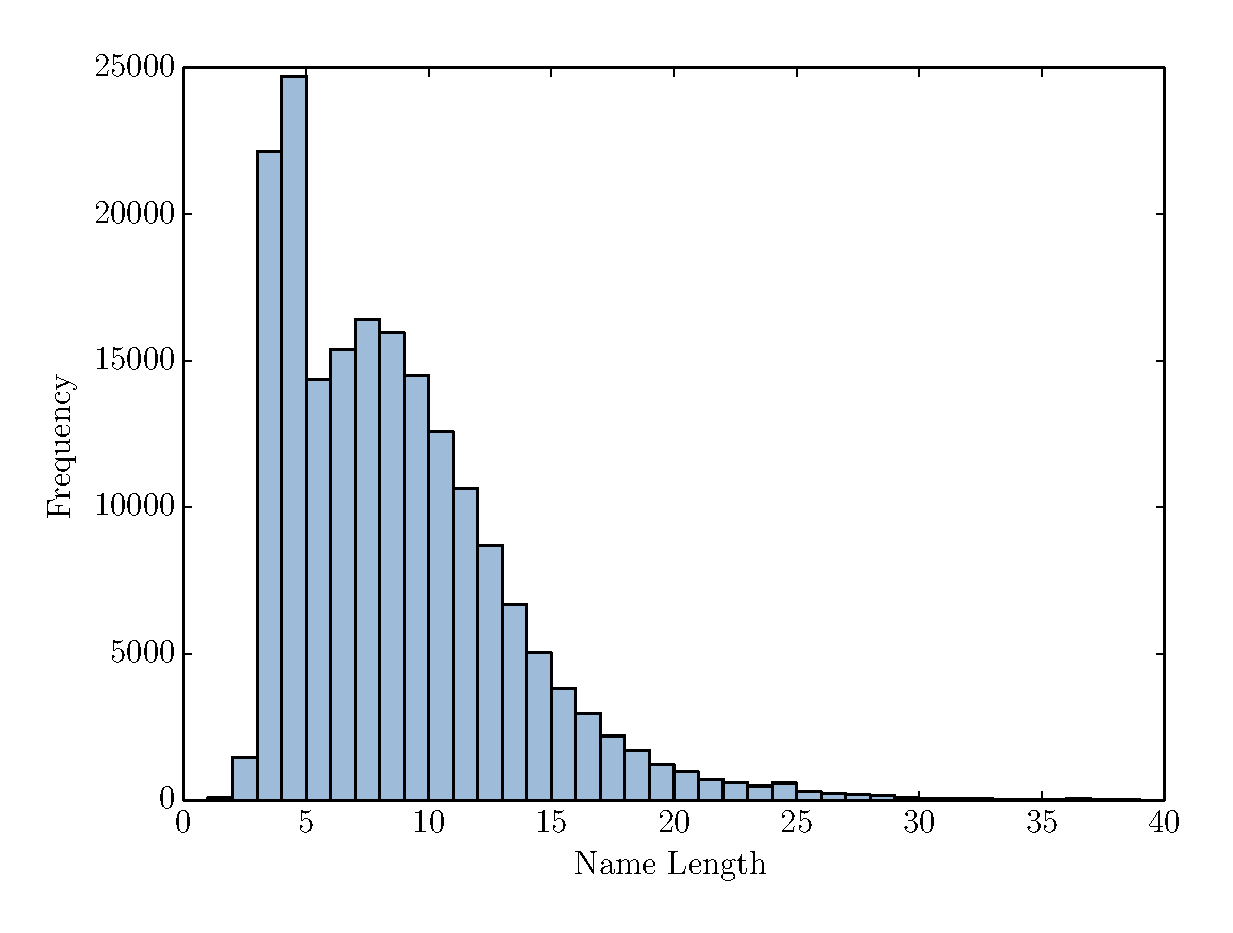
\includegraphics[width=\columnwidth]{figures/name_length_histogram}
  \caption{The number of Namecoin names registered as a function of name length.}
  \label{fig:name_length_histogram}
\end{figure}

\begin{table}
\begin{tabular}{l | c | c }
Length & Number available & Percent available \\ \hline
1           & 0                & 0\%  \\
2           & 0                & 0\% \\
3           & 14335            & 41.39\% \\
4           & 1268585          & 99.00\% \\
5           & 47401012         & 99.97\% \\
$\vdots$    & $\vdots$         & $\vdots$
\end{tabular}
\caption{Availability of names availably by length given in an absolute count, and as a percent of all legal names. All possible names are counted combinatorially using the rules given by \cite{bitdnsspec}.}
\label{table:names_available}
\end{table}